%
% This is a template for the cs_thesis.sty.
%
%
\documentclass[12pt]{report}
\usepackage{cs_thesis}
\usepackage[pdftex]{graphicx}
\usepackage[utf8]{inputenc}
\usepackage{amsmath}

\title{LEARNING LIKE A HUMAN IN COGNITIVE ROBOT \\ LITERATURE SURVEY REPORT}


\author{Semih Onay}
\program{Computer Science}

\supervisor{Assistant Professor Elena Battini Sönmez}


\begin{document}

\makecstitle

\chapter{INTRODUCTION}
\pagenumbering{arabic}

\section{Can we teach languages to a robot like us ?}

Traditional way of learning in robots are known as machine learning.The process which gathers information around itself with sensors and feedbacks and robot trains it self with given sample data sets then interprets it from these data sets and makes estimations.

In Figure 1.1 it shows a different way of learning like our brain structure using neural networks.

\begin{figure}[h]
\begin{center}
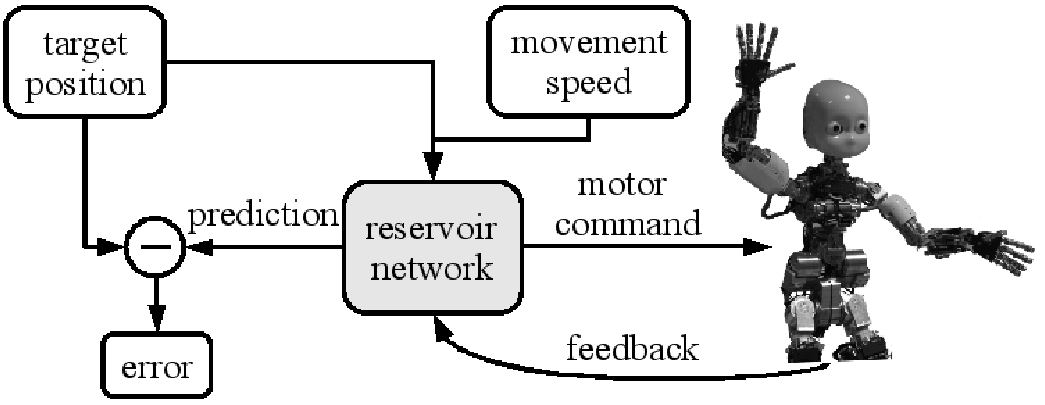
\includegraphics[scale=0.5]{controller.png}
\caption{Neural Learning Method}
\end{center}
\end{figure}

\chapter{RESEARCH AIM AND OBJECTIVES}
\section{What are we going to do ?}

\begin{itemize}
	\item To understand how cognitive model for robots work
	\item To demonstrate and measure cognitive methods
	\item To extend known words,sentences to many and be able to implement correctly
\end{itemize}


\subsection{What We Will Use}

We won't be able to use iCub robot to demonstrate and apply our work.We will use iCub simulation on YARP (Yet Another Robot Platform) to measure and implement our methods.

\chapter{RESOURCES}

\begin{enumerate}
	\item THRIVE: Trust in Human Robot Interaction Via Embodiment,Professor Angelo Cangelosi
Centre for Robotics and Neural Systems, Plymouth University, UK
	\item The grounding of higher order concepts in action and language: A cognitive robotics model, Francesca Stramandinoli, Davide Marocco, Angelo Cangelosi
	\item Towards the Grounding of Abstract Words: A Neural Network Model for Cognitive Robots, Francesca Stramandinoli, Angelo Cangelosi and Davide Marocco

\end{enumerate}
%\appendix

%\chapter{TITLE OF THE FIRST APPENDIX}

\begin{thebibliography}{9}
\bibitem{diagram} Figure.1.1 : http://www.cor-lab.de/content/cognitive-robotics-and-learning

\end{thebibliography}
\end{document}
